% TODO

% SOURCE: \cite{deepComplexNetworks}
% - motivation for completely complex networks

\begin{figure}[htbp]
    \centering
    \makebox[\textwidth][c]{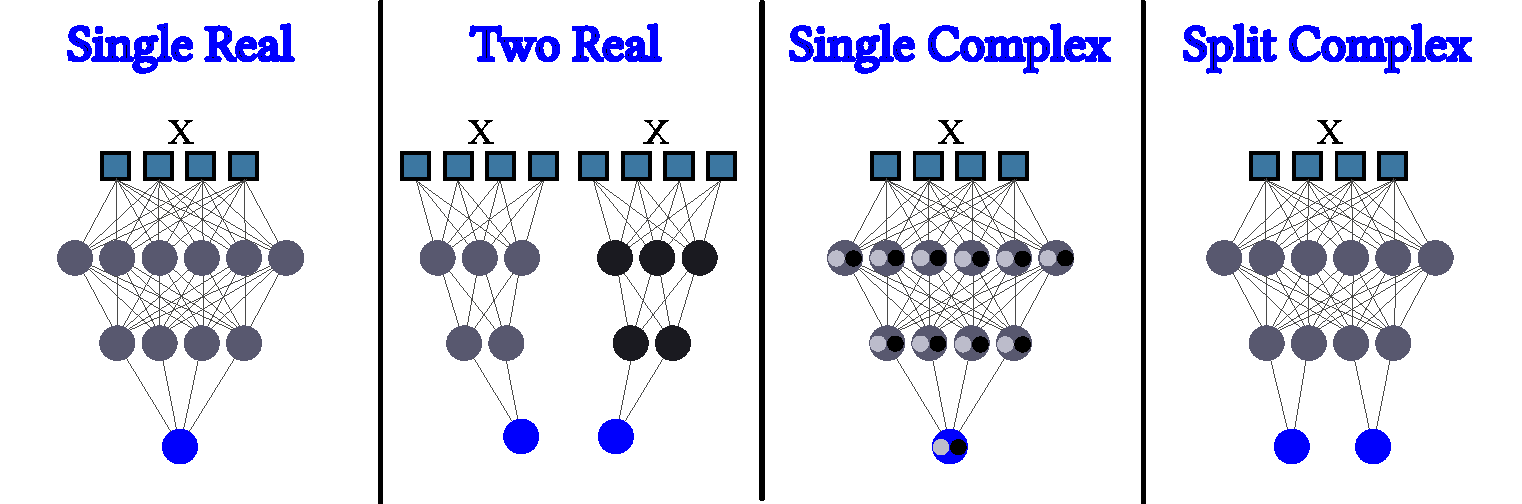
\includegraphics[width=1\textwidth]{./experiments/ground-state-search/ansatz/ansatz.pdf}}
    \caption{
        Schematic visualization of how the four different possibilities for the ansatz are implemented.
        \emph{Single Real} gives a pure real wavefunction output. The architecture is a single network with only real parameters.
        \emph{Two Real} gives a complex wavefunction output (two real numbers, one for the phase and one for the amplitude). The architecture consists of two half-size networks with only real parameters. They do not interact.
        \emph{Single Complex} gives a complex wavefunction output (directly one complex type number). The architecture is a single network with every parameter being a complex number.
        \emph{Split Complex} gives a complex wavefunction output (two real numbers, one for the phase and one for the amplitude). The architecture is a single network with only real parameters, but at the last stage it is split to give two outputs instead of one. The difference to the two real ansatz is that the two \glqq halves\grqq{} of the network can interact.
    }
    \label{fig:ansatz-comparisons}
    
    \makebox[\textwidth][c]{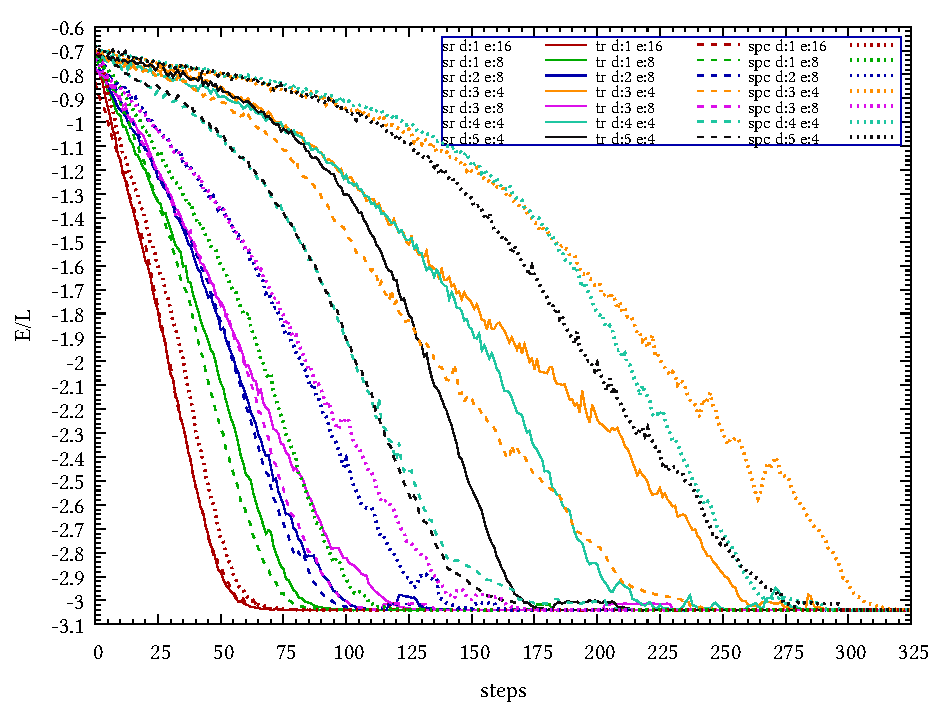
\includegraphics[width=1.1\textwidth]{./experiments/ground-state-search/ansatz/hyperparameter-matrix/hyperparameter-matrix.pdf}}
    \caption{Comparison of hyperparameter combinations. 
            The ansatz is encoded in the dash type, the color specifies the metaformer hyperparameters.
            \emph{sr d:1 e:8} meaning single-real, depth 1 and embed-dimension 8.
            All datasets have been calculated for a randomly encoded \emph{trigonal\_square} lattice with 64 lattice sites.
            Every model is of the type \emph{GPF-NNN} with a mlp-ratio of 4. The Ising parameters are $J=-1$ and $h=-0.7$.
    }
    \label{fig:hyperparameter-matrix}
\end{figure}